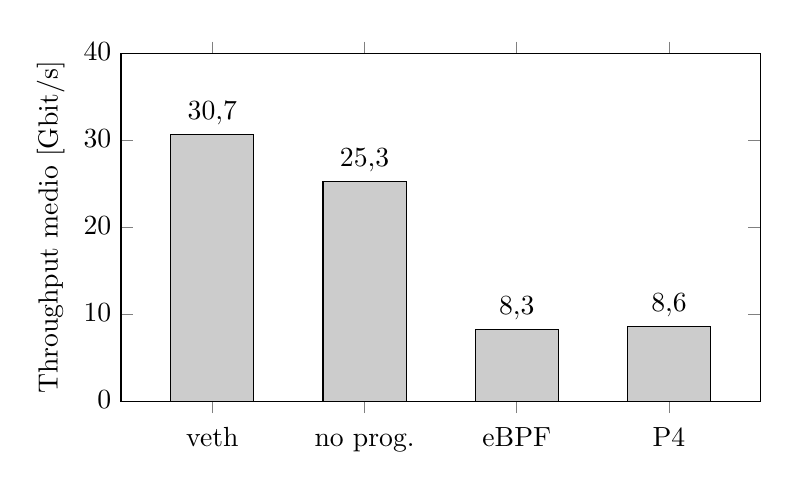
\begin{tikzpicture}
\begin{axis}[
    ybar,
    width=0.8\textwidth, height=6cm,
    symbolic x coords={veth, noprog, ebpf, p4},
    xtick=data,
    typeset ticklabels with strut,
    xticklabels={veth, no prog., eBPF, P4},
    ylabel={Throughput medio [Gbit/s]},
    ymin=0, ymax=40,
    bar width=30pt,
    enlarge x limits=0.2,
    nodes near coords,
    nodes near coords style={/pgf/number format/.cd, fixed, precision=1, use comma},
]
\addplot[fill=gray!40, draw=black] coordinates {(veth,30.7) (noprog,25.3) (ebpf,8.3) (p4,8.6)};
\end{axis}
\end{tikzpicture}
